\section{Economic Analysis}
\subsection{Project description}
Spending Tracker is an application developed for different target groups,for young people which face problems at the chapter of correct money management and as well for older people,who want to monitor all expenses,such as it's user interface is very clear and simple to use for all groups of people in the society.The main task of the application is scanning the receipts and displaying the total expenses for different periods,depending on user's choice,and for different stores,which present categories in the statistics bar chart.Such as it does not require a manual input introducing, it presents a major advantage for its users.This application ensures managements of two most important values in the life: money and time.It saves time by offering that simple possibility of scanning the receipt, and it saves money of course because the main purpose of the application is tracking right the budget,by monitoring day by day all the expenses,and making some decisions according the correctness of their spending.

It is worth mentioning that such applications already exist on the market but they're lack of the most functionality the Spending Tracker has,automatic receipt scanner by taking a photo of the receipt.Also,it's strong point is the simplicity in use,it does not require connection to a bank account or other dubious actions as can be observed in other existing applications on market.It offers exactly what needs every person,nothing more,a user friendly interface and a quick result displaying.

Before proceeding to the implementation of the system,it is necessary to analyse the project budget,this will help to find a justifiable economical point of view over the system.In order to understand and decide if the product is workable on the national market,it would be better to elaborate an overview of the expenditures and incomes after releasing the application.Given that fact,the economic analysis should be one of the first steps in starting development of any product,whose final result would be a general overview on the elaboration of the system.

This chapter represents the analysis of all expenses necessary to elaborate the application,starting from  materials/non-materials used for long term, time schedule establishment and indirect expenses. After that,the days necessary for development should be estimated,should be established the working team and of course each team member salary.Only after this starting analysis will be clear what steps should be performed further in order to have a gain.Even this chapter is last,it is in fact the most important one in real life,because economic analysis is a means to help bring about a better allocation of resources that can lead to enhanced incomes for investment or consumption purposes,it is best undertaken at the early stages of the project cycle to enable decision makers to make an informed decision on whether to undertake a particular investment given various alternatives and their corresponding costs.

\newpage
\addtocontents{toc}{\protect\newpage}
\subsection{Project time schedule}
Taking into account that the Spending Tracker application is quite complex and have in the requirements list many features to be implemented,it would be better to plan a time schedule.In order to get the better results faster,and also a considerable income,will be tried to be used \textbf{Agile Software Development}.In such a way the product will be delivered faster,maybe not implemented at all,a process of frequent feedbacks will be adopted for excluding risks of a single-pass development when all the requirements are implemented.The future modifications can be treated as improvements for the base application which represents a benefit of Agile.
\subsubsection{SWOT Analysis}
The SWOT analysis(Strengths,Weaknesses,Opportunities,Threats) are very suitable for analysing the system before starting the implementation,such as it gives a brief overview about expectations or possible problems that can appear during the lifetime of the system.They can inform later steps in planning to achieve the expected objectives.By understanding the weaknesses of the product, threats can be managed and eliminated that would otherwise catch the unawares.Bellow is represented the strategic planning method, used to evaluate Strengths, Weaknesses, Opportunities and Threads that can involve the given system.
\begin{figure}[H]
	\centering
	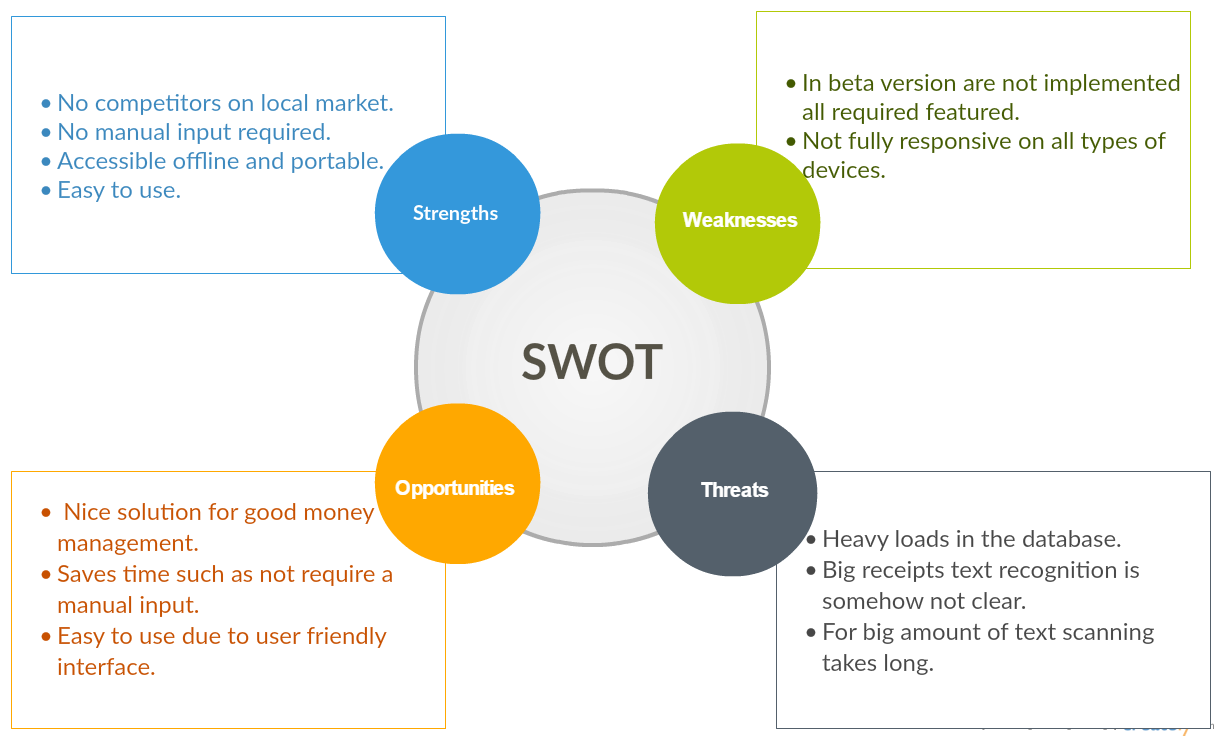
\includegraphics[width=18cm]{Chapter4/img1.png}
	\caption{SWOT Analysis}
	\label{fig:SWOT Analysis}
\end{figure}
\newpage
Referring to the SWOT analysis,the most important factors which can affect the product can be detected.However the SWOT analysis does not necessarily offer solutions.They only allow people at the earliest stage of development to understand better the business, to address weaknesses,detect threads,take advantage of the strengths,develop business goals and strategies for achieving them.
\subsubsection{Defining objectives}
The main objective of the project is to improve the personal budget management for all types of users, meaning different categories of ages and working domains.Also as it will be most based on local environment, meaning local stores,its purpose is to spread among the society.As the application is provided as free product,it is expected to gain users very quickly.
\subsubsection{Time schedule establishment}
There are some steps to be performed in order to reach the final result of Spending Tracker application:
\begin{itemize}
	\item \textbf{Planning} - Form some ideas about the design of the project, build some sketches and diagrams, determine amount of needed resources.
	\item \textbf{Analysis} - This step is about analysing the performance of the software at various stages and making notes on additional requirements.
	\item \textbf{Design} - Building the architecture of the project.
	\item \textbf{Development} - Creating the application itself,based on the initial requirements.
	\item \textbf{Testing} - This can be done by performing debugging,in order to ensure the correctness of the functionality,also at this step is done manual testing.
	\item \textbf{Maintenance} - Once the software passes through all the stages without any issues, it is to undergo a maintenance process wherein it will be maintained and upgraded from time to time to adapt to changes.
\end{itemize}
A key initial task for the project management team is to prepare a proper timetable which will set a concise deadline for every step enumerated above.Of course,the planning period can be considered a flexible one such as changes are allowed at this step during all life cycle of the project if it's necessary. In the Table 4.1 are represented all the general steps involving the development of the project. The following annotations were used: PM – Project Manager, BA - Business Analyst, D - Designer,BD – Back-End Developer, QA  - Quality Assurance Engineer.

\begin{table}[H]
	\centering
	\caption{Time schedule}
	\label{Time schedule}
	\begin{tabular}{|l|l|c|l|}
		\hline
		\textbf{Nr.} & \textbf{Activity Name}                              & \multicolumn{1}{l|}{\textbf{Duration (days)}} & \textbf{People involved} \\ \hline
		1            & Planning requirments and activities schedule        & 7                                             & PM,BA                    \\ \hline
		2            & Perform market analysis                             & 5                                             & PM                       \\ \hline
		3            & Writing Business Requirment Document                & 5                                             & BA                       \\ \hline
		4            & Elaborate UML diagrams                              & 3                                             & PM,BD                    \\ \hline
		5            & Building application design                         & 5                                             & D                        \\ \hline
		6            & Implementing back-end functionality                 & 21                                            & BD                       \\ \hline
		7            & Testing application                                 & 7                                             & QA                       \\ \hline
		8            & Bug fixing process                                  & 7                                             & BD                    \\ \hline
		9            & Bugs verification process                                  & 2                                             & QA                    \\ \hline
		10           & Writing documentation                               & 2                                             & BA,BD                 \\ \hline
		11           & Production realese                                  & 1                                             & PM,BA,BD,QA              \\ \hline
		12           & Feedback / Maintance                                & -                                             & PM,BD                    \\ \hline
		13           & \textbf{Total time required for system development} & \textbf{73}                                   &                          \\ \hline
	\end{tabular}
\end{table}
The table above presents a sketch for the first beta version of the application.Each activity was estimated in time and in human resources as well.For the beta version of the Spending Tracker application was estimated a total volume of 73 working days.There are 6 specialists supposed to work on project:
\begin{itemize}
	\item Project Manager (PM) - 16 days
	\item Business Analyst (BA) - 8 days
	\item Designer (D) - 5 days
	\item Back-End Developer (BD) - 31 days
	\item Quality Assurance Engineer (QA) - 10 days
\end{itemize}
Above is represented the approximate amount of spent time for each specialist.
\subsection{Economic motivation}
Establishing economical motivation is a natural process for the IT projects, such as it is based on several key points which should be taken in consideration as are concurrences in economic relationships and social needs, which suppose  a wide research space. Taking into account the conditions of a low degree of determination of the marketing environment, of high prices’ volatility, a common business-plan doesn’t allow the exact foreseeing of the final results of the business. In this context, one of the basic instruments are considered choosing the methods, the right positions and index for the economical proofs. Realization of this goal conditions a large number of scientifically research, subordinated to the primary goal and formulated by means of the following objectives:
\begin{itemize}
	\item  Studying the theoretical and methodical aspects of the business-planning in the conditions of the concurrency on the market;
	\item Systematization, determining the methodology and specifying the index for the economical proof of the business-plans in IT;
	\item Study and analysis of the actual practice of economical proofs of the business-plans for IT in Republic of Moldova;
	\item Developing methodological concepts of the proofs of the decision of investment in the conditions of risk and incertitude;
	\item Studying the evaluation criteria of the business-projects’ efficiency and elaboration of a mechanism of complex evaluation of these.
\end{itemize}
\subsubsection{Tangible and intangible asset expenses}
Spendings and initial budget are the key factors which are met at the very beginning of the project,by imposing some limitations on the complexity of the system and defining its boundaries.This chapter describes the evaluation of approximate amount of money needed for the development of Spending Tracker application,in order to ensure the correct management of financial resources.For the beginning in the Table 4.2 will be listed all the physical stuff used for the project.Touchable assets are defined as any assets that have a physical form.
\begin{table}[H]
	\centering
	\caption{Tangible assets}
	\label{Tangible assets}
	\resizebox{\textwidth}{!}{%
	\begin{tabular}{|l|l|l|l|l|l|}
		\hline
		\textbf{Material} & \textbf{Specification} & \textbf{Measurement unit} & \textbf{Price per unit(MDL)} & \textbf{Quantity} & \textbf{Sum(MDL)} \\ \hline
		HP Pavillion      & AMD processor          & Unit                   & 9000                       & 6              & 54000             \\ \hline
		Samsung Galaxy A5      & Android minimum API level 15         & Unit                   & 7800                       & 1              & 7800              \\ \hline
		\multicolumn{5}{|r|}{Total}                                                                                       & 61800             \\ \hline
	\end{tabular}}
\end{table}
The tangible assets were estimated to 6 HP Pavillion laptops, for each member in the team, for not holding work, and one Samsung Galaxy A5 mobile phone, for debugging the application.Bellow in the Table 4.3 are presented all intangible assets which mean all those that do not process a physical form.So, this table will represent all the software needed for building the application and costs for the licences.
\begin{table}[H]
	\centering
	\caption{Intangible assets}
	\label{Intangible assets}
	\resizebox{\textwidth}{!}{%
	\begin{tabular}{|l|l|l|l|l|l|}
		\hline
		\textbf{Material} & \textbf{Specification}        & \textbf{Measurement unit} & \textbf{Price per unit(MDL)} & \textbf{Quantity} & \textbf{Sum(MDL)} \\ \hline
		Licence          & Enterprise Architect  & Unit                   & 1800                       & 1              & 1800              \\ \hline
		Account           & Google Play Developer Console & Unit                   & 470                        & 1              & 470               \\ \hline
		\multicolumn{5}{|r|}{Total}                                                                                              & 2270              \\ \hline
	\end{tabular}}
\end{table}
First of all the licence for Enterprise Architect Desktop Edition is needed in planning requirements stage, when modelling the architecture of the system.Android Studio IDE used for development is free, so no licence is needed for it.Finally for deploying the application on Play Store, a Google Play Developer Console account is needed.
There are other additional expenses which should be taken in account as well.They represent the direct expenses used for work facilitation during project development.The Table 4.4 represents the direction expenses:
\begin{table}[H]
	\centering
	\caption{Direct expenses}
	\label{my-label}
	\resizebox{\textwidth}{!}{%
	\begin{tabular}{|l|l|l|l|l|l|}
		\hline
		\textbf{Material} & \textbf{Specification}    & \textbf{Mesurement unit} & \textbf{Price per unit(MDL)} & \textbf{Quantity} & \textbf{Sum(MDL)} \\ \hline
		Whiteboard        & Universal Dry Erase Board & Unit                     & 700                          & 1                 & 700               \\ \hline
		Paper             & A4                        & 100 sheets               & 60                           & 1                 & 60                \\ \hline
		Pen               & Black pen                 & Unit                     & 7                            & 5                 & 35                \\ \hline
		\multicolumn{5}{|r|}{Total}                                                                                                 & 795               \\ \hline
	\end{tabular}}
\end{table}
Summing up all the expenses from all three tables can be calculated the approximate total amount of expenses for Spending Tracker application.
\begin{equation}
T_{e} = 61800 + 2270 + 795 = 64865
\end{equation}
\subsubsection{Salary expenses}
In this chapter it's time to discuss the remuneration of each employee during the process of development.Let's assume the following salaries per day for each specialist:
\begin{itemize}
	\item Project Manager - 500 MDL per day
	\item Business Analyst - 400 MDL per day
	\item Designer - 300 MDL per day
	\item Back-End Developer - 500 MDL per day
	\item Quality Assurance Engineer - 400 MDL per day
\end{itemize}
Given the above information can be built the table of the expenses for human resources for the whole project.
\begin{table}[H]
	\centering
	\caption{Salary expenses}
	\label{Salary expenses}
	\begin{tabular}{|l|l|l|l|}
		\hline
		\textbf{Employee}          & \textbf{Working days} & \textbf{Salary per day(MDL)} & \textbf{Salary fund(MDL)} \\ \hline
		Project Manager            & 16                    & 500                          & 8000                      \\ \hline
		Business Analyst           & 8                     & 400                          & 3200                      \\ \hline
		Designer                   & 5                     & 300                          & 1500                      \\ \hline
		Back-End Developer         & 31                    & 500                          & 15500                     \\ \hline
		Quality Assurance Engineer & 10                    & 400                          & 4000                      \\ \hline
		\multicolumn{3}{|r|}{Total}                                                       & 32200                     \\ \hline
	\end{tabular}
\end{table}
The social services fund should not be forgotten such as from the total salary fund a part of money is retrieved.According \url{https://salarii.md/} where can be found all taxes for the current year, can be observed that the social fund constitutes 23\%, medical assurance - 4.5\%.Bellow is computed the social service fund, according the relation (4.2):
\begin{equation}
\label{eq:sf}
\begin{split}
FS  &= F_{re} \cdot T_{fs} \\
	&= 32200 \cdot 0.23  \\	
	&= 7406,
\end{split}
\end{equation}
\noindent
where FS means salary expense, $F_{re}$ represent the salary expense fund and $T_{fs}$ is the social service tax which is approved each year.The medical assurance fund is computed bellow:
\begin{equation}
\begin{split}
MI  &= F_{re} \cdot T_{mi}\\ 
	&= 32200 \cdot 0.045\\ 
	&= 1149,
\end{split}
\end{equation}
where $T_{mi}$ is the mandatory medical insurance tax also approved each year by the law of medical insurance.
So, the total expense fund is calculated as sum of all calculated indicators:
\begin{equation}
WEF = F_{re} + FS + MI = 
32200 + 7406 + 1149 = 40775,
\end{equation}
where $WEF$ is the work expense fund,$FS$ is the social fund and $MI$ is the medical insurance fund.The final result shows the total work expense fund.
\subsection{Individual person salary}
\subsubsection{Indirect expenses}
\subsubsection{Wear and depreciation}
\subsubsection{Product cost}
\subsubsection{Economic indicators and results}
\subsection{Economic conclusions}